\chapter{Resultados (Ejemplos de gráficas)}
\label{ch:resultados}

En este capítulo se presentan los resultados obtenidos mediante diferentes pruebas de \gls{throughput} y \gls{latencia}. Se muestran ejemplos de cómo crear gráficas con \LaTeX{} usando el paquete \texttt{pgfplots}.

\section{Gráficas con PGFPlots}
\label{sec:graficas-pgfplots}

PGFPlots es un paquete potente para crear gráficas directamente en \LaTeX{}. Permite generar visualizaciones de alta calidad que se integran perfectamente con el estilo tipográfico del documento.

\subsection{Gráfica de líneas}
\label{subsec:grafica-lineas}

Las gráficas de líneas son ideales para mostrar tendencias temporales o relaciones continuas entre variables.

\begin{figure}[H]
  \centering
  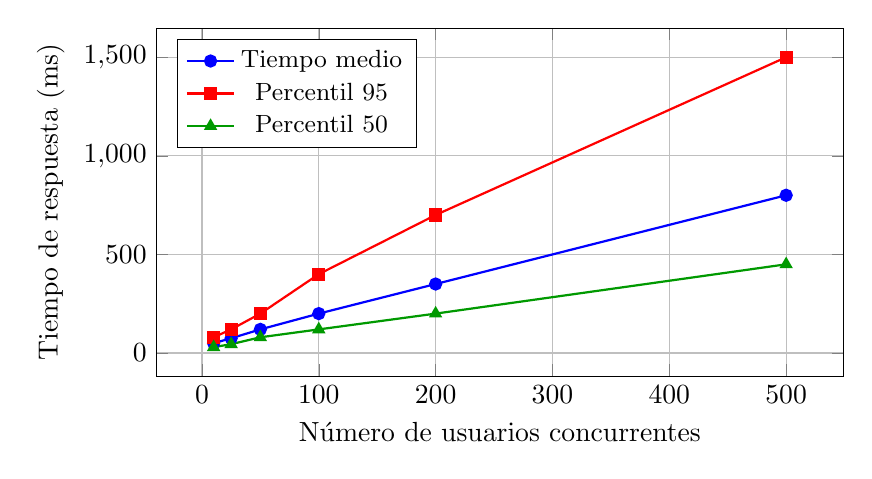
\begin{tikzpicture}
    \begin{axis}[
      xlabel={Número de usuarios concurrentes},
      ylabel={Tiempo de respuesta (ms)},
      grid=major,
      width=0.85\textwidth,
      height=6cm,
      legend pos=north west,
      legend style={font=\small},
    ]
    \addplot[blue, mark=*, thick] coordinates {
      (10, 50) (25, 75) (50, 120) (100, 200) (200, 350) (500, 800)
    };
    \addlegendentry{Tiempo medio}

    \addplot[red, mark=square*, thick] coordinates {
      (10, 80) (25, 120) (50, 200) (100, 400) (200, 700) (500, 1500)
    };
    \addlegendentry{Percentil 95}

    \addplot[green!60!black, mark=triangle*, thick] coordinates {
      (10, 30) (25, 45) (50, 80) (100, 120) (200, 200) (500, 450)
    };
    \addlegendentry{Percentil 50}
    \end{axis}
  \end{tikzpicture}
  \caption{Tiempos de respuesta según carga de usuarios}
  \label{fig:rendimiento}
\end{figure}

Como se observa en la Figura~\ref{fig:rendimiento}, el sistema mantiene tiempos de respuesta aceptables incluso con 200 usuarios concurrentes.

\subsection{Gráfica de barras}
\label{subsec:grafica-barras}

Las gráficas de barras permiten comparar valores discretos entre categorías.

\begin{figure}[H]
  \centering
  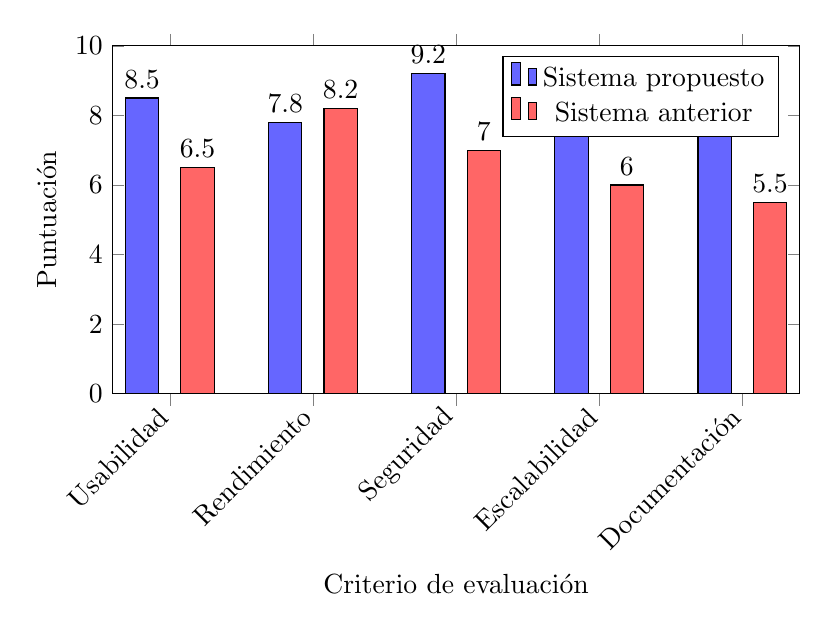
\begin{tikzpicture}
    \begin{axis}[
      ybar=8pt,
      width=0.85\textwidth,
      height=6cm,
      ylabel={Puntuación},
      xlabel={Criterio de evaluación},
      symbolic x coords={Usabilidad, Rendimiento, Seguridad, Escalabilidad, Documentación},
      xtick=data,
      x tick label style={rotate=45, anchor=east},
      ymin=0,
      ymax=10,
      bar width=12pt,
      legend pos=north east,
      nodes near coords,
      nodes near coords align={vertical},
    ]
    \addplot[fill=blue!60] coordinates {
      (Usabilidad, 8.5)
      (Rendimiento, 7.8)
      (Seguridad, 9.2)
      (Escalabilidad, 7.5)
      (Documentación, 8.0)
    };
    \addlegendentry{Sistema propuesto}

    \addplot[fill=red!60] coordinates {
      (Usabilidad, 6.5)
      (Rendimiento, 8.2)
      (Seguridad, 7.0)
      (Escalabilidad, 6.0)
      (Documentación, 5.5)
    };
    \addlegendentry{Sistema anterior}
    \end{axis}
  \end{tikzpicture}
  \caption{Comparativa de evaluación del sistema}
  \label{fig:barras}
\end{figure}

\subsection{Gráfica circular (pie chart)}
\label{subsec:grafica-circular}

Las gráficas circulares muestran proporciones de un total. Este ejemplo usa el paquete \texttt{pgf-pie}.

\begin{figure}[H]
  \centering
  \begin{tikzpicture}
    \pie[
      text=legend,
      radius=2.5,
      color={blue!60, red!60, green!60, orange!60, purple!60}
    ]{
      35/Desarrollo,
      25/Análisis,
      20/Pruebas,
      12/Documentación,
      8/Reuniones
    }
  \end{tikzpicture}
  \caption{Distribución del tiempo del proyecto}
  \label{fig:pie}
\end{figure}

\subsection{Gráfica de área}
\label{subsec:grafica-area}

Las gráficas de área apiladas son útiles para mostrar la evolución de múltiples series y su contribución al total.

\begin{figure}[H]
  \centering
  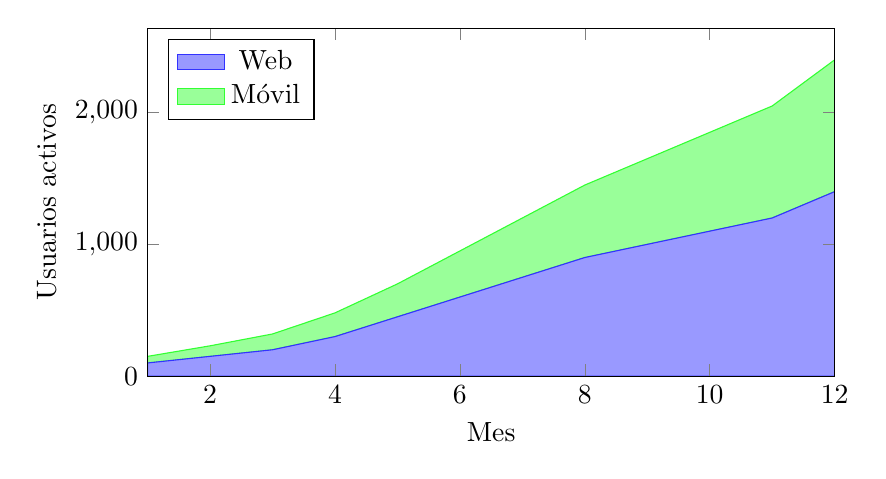
\begin{tikzpicture}
    \begin{axis}[
      width=0.85\textwidth,
      height=6cm,
      xlabel={Mes},
      ylabel={Usuarios activos},
      xmin=1, xmax=12,
      ymin=0,
      area style,
      stack plots=y,
      legend pos=north west,
    ]
    \addplot+[fill=blue!40, draw=blue!80] coordinates {
      (1,100) (2,150) (3,200) (4,300) (5,450) (6,600)
      (7,750) (8,900) (9,1000) (10,1100) (11,1200) (12,1400)
    } \closedcycle;
    \addlegendentry{Web}

    \addplot+[fill=green!40, draw=green!80] coordinates {
      (1,50) (2,80) (3,120) (4,180) (5,250) (6,350)
      (7,450) (8,550) (9,650) (10,750) (11,850) (12,1000)
    } \closedcycle;
    \addlegendentry{Móvil}
    \end{axis}
  \end{tikzpicture}
  \caption{Evolución de usuarios activos por plataforma}
  \label{fig:area}
\end{figure}

\subsection{Gráfica de dispersión}
\label{subsec:grafica-dispersion}

Las gráficas de dispersión permiten visualizar correlaciones entre variables y ajustar líneas de regresión.

\begin{figure}[H]
  \centering
  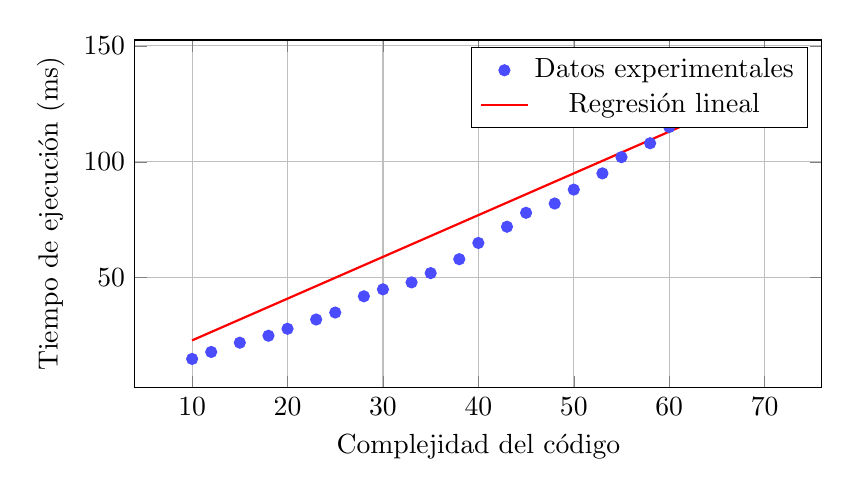
\begin{tikzpicture}
    \begin{axis}[
      width=0.85\textwidth,
      height=6cm,
      xlabel={Complejidad del código},
      ylabel={Tiempo de ejecución (ms)},
      grid=major,
    ]
    \addplot[only marks, mark=*, blue!70, mark size=2pt] coordinates {
      (10,15) (15,22) (20,28) (25,35) (30,45) (35,52)
      (40,65) (45,78) (50,88) (55,102) (60,115) (65,130)
      (12,18) (18,25) (23,32) (28,42) (33,48) (38,58)
      (43,72) (48,82) (53,95) (58,108) (63,122) (68,140)
    };

    \addplot[red, thick, domain=10:70] {1.8*x + 5};
    \addlegendentry{Datos experimentales}
    \addlegendentry{Regresión lineal}
    \end{axis}
  \end{tikzpicture}
  \caption{Correlación entre complejidad y tiempo de ejecución}
  \label{fig:scatter}
\end{figure}

\section{Resultados de la implementación}
\label{sec:resultados-implementacion}

\subsection{Funcionalidades implementadas}
\label{subsec:funcionalidades}

Se han implementado con éxito las siguientes funcionalidades:

\begin{table}[H]
  \centering
  \caption{Estado de implementación de funcionalidades}
  \label{tab:funcionalidades}
  \begin{tabular}{@{}lcc@{}}
    \toprule
    \textbf{Funcionalidad} & \textbf{Estado} & \textbf{Cobertura tests} \\
    \midrule
    Autenticación de usuarios & Completado & 95\% \\
    Gestión de datos & Completado & 88\% \\
    Generación de informes & Completado & 82\% \\
    API REST & Completado & 90\% \\
    Interfaz de usuario & Completado & 75\% \\
    Sistema de caché & Completado & 85\% \\
    \bottomrule
  \end{tabular}
\end{table}

\subsection{Consumo de recursos}
\label{subsec:consumo-recursos}

El consumo de memoria se mantiene estable, como muestra la siguiente ecuación para el consumo estimado:

\begin{equation}
  M_{total} = M_{base} + n \cdot M_{usuario}
  \label{eq:memoria}
\end{equation}

\begin{condiciones}
  M_{total} & = & memoria total consumida (MB) \\
  M_{base}  & = & memoria base del sistema (256 MB) \\
  n         & = & número de usuarios activos \\
  M_{usuario} & = & memoria por usuario (2.5 MB)
\end{condiciones}

\section{Análisis de resultados}
\label{sec:analisis-resultados}

\subsection{Cumplimiento de objetivos}
\label{subsec:cumplimiento-objetivos}

En la Tabla~\ref{tab:objetivos} se muestra el grado de cumplimiento de cada objetivo:

\begin{table}[H]
  \centering
  \caption{Cumplimiento de objetivos}
  \label{tab:objetivos}
  \begin{tabular}{@{}lp{6cm}c@{}}
    \toprule
    \textbf{Objetivo} & \textbf{Descripción} & \textbf{Cumplimiento} \\
    \midrule
    OE1 & Análisis del estado actual & 100\% \\
    OE2 & Diseño de arquitectura escalable & 100\% \\
    OE3 & Implementación de componentes & 95\% \\
    OE4 & Evaluación del sistema & 100\% \\
    OE5 & Documentación completa & 100\% \\
    \bottomrule
  \end{tabular}
\end{table}

\subsection{Métricas de rendimiento}
\label{subsec:metricas-rendimiento}

\begin{table}[H]
  \centering
  \caption{Métricas de rendimiento del sistema}
  \label{tab:metricas}
  \begin{tabular}{@{}lccc@{}}
    \toprule
    \textbf{Métrica} & \textbf{Objetivo} & \textbf{Resultado} & \textbf{Estado} \\
    \midrule
    Tiempo de respuesta medio & < 200 ms & 145 ms & \textcolor{green!60!black}{\ensuremath{\checkmark}} \\
    Tiempo de respuesta P95 & < 500 ms & 380 ms & \textcolor{green!60!black}{\ensuremath{\checkmark}} \\
    Throughput & > 1000 req/s & 1250 req/s & \textcolor{green!60!black}{\ensuremath{\checkmark}} \\
    Disponibilidad & > 99.5\% & 99.8\% & \textcolor{green!60!black}{\ensuremath{\checkmark}} \\
    Uso de CPU (promedio) & < 70\% & 45\% & \textcolor{green!60!black}{\ensuremath{\checkmark}} \\
    Uso de memoria & < 80\% & 62\% & \textcolor{green!60!black}{\ensuremath{\checkmark}} \\
    \bottomrule
  \end{tabular}
\end{table}

\section{Ejemplo de gráfica 3D}
\label{sec:grafica-3d}

PGFPlots también permite crear gráficas tridimensionales:

\begin{figure}[H]
  \centering
  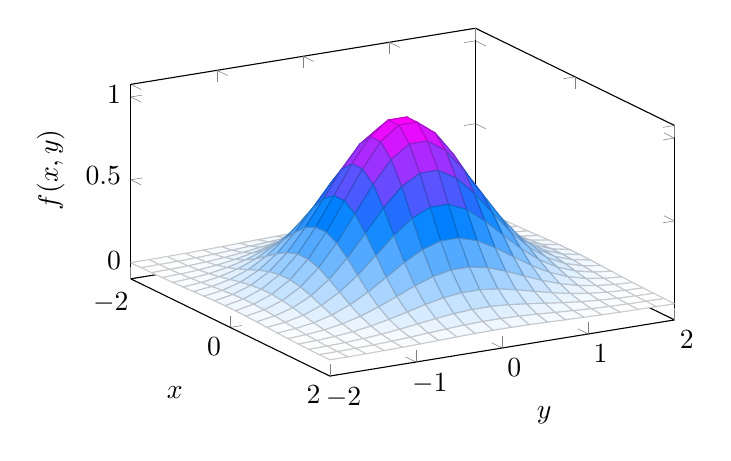
\begin{tikzpicture}
    \begin{axis}[
      width=0.7\textwidth,
      height=6cm,
      view={60}{30},
      xlabel=$x$,
      ylabel=$y$,
      zlabel={$f(x,y)$},
      colormap/cool,
    ]
    \addplot3[
      surf,
      samples=20,
      domain=-2:2,
    ] {exp(-x^2-y^2)};
    \end{axis}
  \end{tikzpicture}
  \caption{Superficie gaussiana $f(x,y) = e^{-x^2-y^2}$}
  \label{fig:3d}
\end{figure}

\section{Exportar gráficas desde herramientas externas}
\label{sec:exportar-graficas}

También es posible exportar gráficas desde otras herramientas:

\begin{itemize}
  \item \textbf{MATLAB:} Usar \texttt{matlab2tikz} para exportar figuras
  \item \textbf{Python (matplotlib):} Usar \texttt{tikzplotlib}
  \item \textbf{R:} Usar el paquete \texttt{tikzDevice}
  \item \textbf{GeoGebra:} Exportar directamente a TikZ
\end{itemize}

\begin{verbatim}
% En MATLAB:
plot(x, y);
matlab2tikz('figura.tex');

% En LaTeX:
\begin{figure}[H]
  \centering
  \input{figuras/figura.tex}
  \caption{Gráfica importada de MATLAB}
\end{figure}
\end{verbatim}

\section{Gráficas con marcadores y anotaciones}
\label{sec:graficas-marcadores}

\subsection{Gráfica con marcadores sobre puntos específicos}
\label{subsec:marcadores-puntos}

\begin{figure}[H]
  \centering
  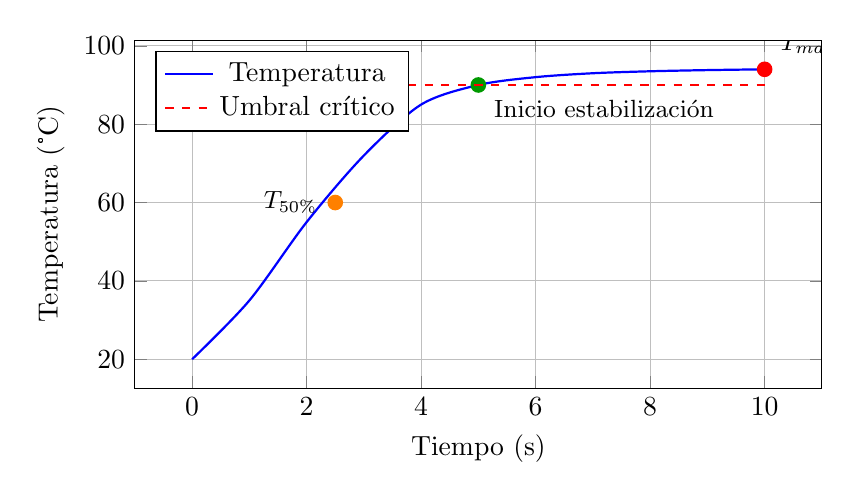
\begin{tikzpicture}
    \begin{axis}[
      width=0.85\textwidth,
      height=6cm,
      xlabel={Tiempo (s)},
      ylabel={Temperatura (°C)},
      grid=major,
      legend pos=north west,
    ]
    % Curva principal
    \addplot[blue, thick, smooth] coordinates {
      (0,20) (1,35) (2,55) (3,72) (4,85) (5,90) (6,92) (7,93) (8,93.5) (9,93.8) (10,94)
    };
    \addlegendentry{Temperatura}

    % Marcadores con anotaciones
    \node[circle, fill=red, inner sep=2pt, label={above right:\small $T_{max}=94°C$}] at (axis cs:10,94) {};
    \node[circle, fill=green!60!black, inner sep=2pt, label={below right:\small Inicio estabilización}] at (axis cs:5,90) {};
    \node[circle, fill=orange, inner sep=2pt, label={left:\small $T_{50\%}$}] at (axis cs:2.5,60) {};

    % Línea de referencia
    \addplot[dashed, red, thick] coordinates {(0,90) (10,90)};
    \addlegendentry{Umbral crítico}
    \end{axis}
  \end{tikzpicture}
  \caption{Curva de calentamiento con puntos críticos marcados}
  \label{fig:marcadores}
\end{figure}

\subsection{Gráfica con barras de error}
\label{subsec:barras-error}

\begin{figure}[H]
  \centering
  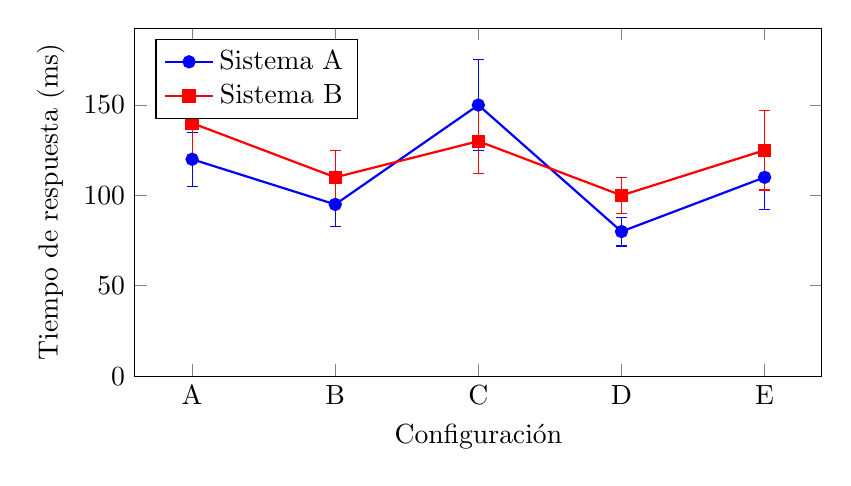
\begin{tikzpicture}
    \begin{axis}[
      width=0.85\textwidth,
      height=6cm,
      xlabel={Configuración},
      ylabel={Tiempo de respuesta (ms)},
      symbolic x coords={A, B, C, D, E},
      xtick=data,
      ymin=0,
      legend pos=north west,
    ]
    % Datos con barras de error
    \addplot[
      blue,
      mark=*,
      thick,
      error bars/.cd,
      y dir=both,
      y explicit,
    ] coordinates {
      (A, 120) +- (0, 15)
      (B, 95) +- (0, 12)
      (C, 150) +- (0, 25)
      (D, 80) +- (0, 8)
      (E, 110) +- (0, 18)
    };
    \addlegendentry{Sistema A}

    \addplot[
      red,
      mark=square*,
      thick,
      error bars/.cd,
      y dir=both,
      y explicit,
    ] coordinates {
      (A, 140) +- (0, 20)
      (B, 110) +- (0, 15)
      (C, 130) +- (0, 18)
      (D, 100) +- (0, 10)
      (E, 125) +- (0, 22)
    };
    \addlegendentry{Sistema B}
    \end{axis}
  \end{tikzpicture}
  \caption{Comparativa de rendimiento con intervalos de confianza}
  \label{fig:errorbars}
\end{figure}

\subsection{Gráfica con área sombreada (intervalo de confianza)}
\label{subsec:area-confianza}

\begin{figure}[H]
  \centering
  \begin{tikzpicture}
    \begin{axis}[
      width=0.85\textwidth,
      height=6cm,
      xlabel={Iteración},
      ylabel={Precisión (\%)},
      grid=major,
      legend pos=south east,
    ]
    % Área de confianza (sombra)
    \addplot[
      name path=upper,
      draw=none,
    ] coordinates {
      (1,72) (2,78) (3,83) (4,87) (5,90) (6,92) (7,93) (8,94) (9,94.5) (10,95)
    };

    \addplot[
      name path=lower,
      draw=none,
    ] coordinates {
      (1,62) (2,68) (3,73) (4,77) (5,80) (6,82) (7,83) (8,84) (9,84.5) (10,85)
    };

    \addplot[blue!20] fill between[of=upper and lower];

    % Curva media
    \addplot[blue, thick, mark=*, mark size=1.5pt] coordinates {
      (1,67) (2,73) (3,78) (4,82) (5,85) (6,87) (7,88) (8,89) (9,89.5) (10,90)
    };
    \addlegendentry{Media $\pm$ desv. estándar}
    \end{axis}
  \end{tikzpicture}
  \caption{Evolución del entrenamiento con banda de confianza}
  \label{fig:confidence}
\end{figure}

\subsection{Gráfica con múltiples ejes Y}
\label{subsec:multiples-ejes}

\begin{figure}[H]
  \centering
  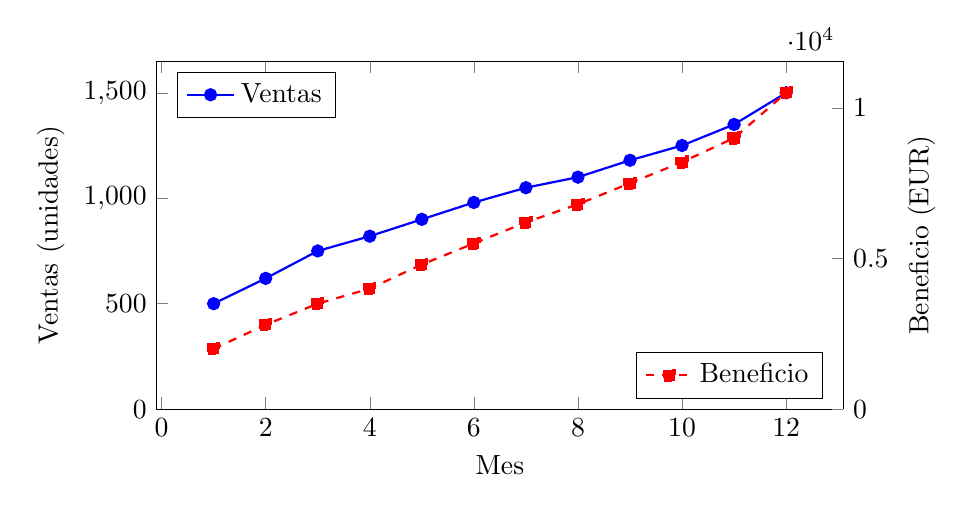
\begin{tikzpicture}
    \begin{axis}[
      width=0.85\textwidth,
      height=6cm,
      xlabel={Mes},
      ylabel={Ventas (unidades)},
      axis y line*=left,
      ymin=0,
      legend pos=north west,
    ]
    \addplot[blue, thick, mark=*] coordinates {
      (1,500) (2,620) (3,750) (4,820) (5,900) (6,980)
      (7,1050) (8,1100) (9,1180) (10,1250) (11,1350) (12,1500)
    };
    \addlegendentry{Ventas}
    \end{axis}

    \begin{axis}[
      width=0.85\textwidth,
      height=6cm,
      ylabel={Beneficio (EUR)},
      axis y line*=right,
      axis x line=none,
      ymin=0,
      legend pos=south east,
    ]
    \addplot[red, thick, mark=square*, dashed] coordinates {
      (1,2000) (2,2800) (3,3500) (4,4000) (5,4800) (6,5500)
      (7,6200) (8,6800) (9,7500) (10,8200) (11,9000) (12,10500)
    };
    \addlegendentry{Beneficio}
    \end{axis}
  \end{tikzpicture}
  \caption{Ventas y beneficios mensuales (doble eje Y)}
  \label{fig:dualaxis}
\end{figure}

\subsection{Gráfica de distribución (histograma)}
\label{subsec:histograma}

\begin{figure}[H]
  \centering
  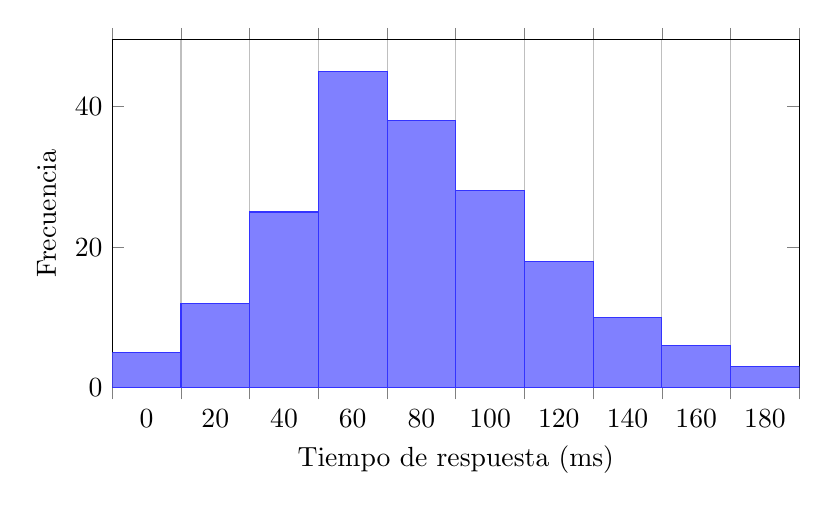
\begin{tikzpicture}
    \begin{axis}[
      width=0.85\textwidth,
      height=6cm,
      ybar interval,
      xlabel={Tiempo de respuesta (ms)},
      ylabel={Frecuencia},
      xmin=0, xmax=200,
      ymin=0,
    ]
    \addplot[fill=blue!50, draw=blue!80] coordinates {
      (0,5) (20,12) (40,25) (60,45) (80,38)
      (100,28) (120,18) (140,10) (160,6) (180,3) (200,0)
    };
    \end{axis}
  \end{tikzpicture}
  \caption{Distribución de tiempos de respuesta}
  \label{fig:histograma}
\end{figure}

\subsection{Gráfica de radar (polígono)}
\label{subsec:grafica-radar}

Las gráficas de radar son útiles para comparar múltiples variables simultáneamente:

\begin{figure}[H]
  \centering
  \begin{tikzpicture}
    \begin{polaraxis}[
      width=8cm,
      xtick={0,60,120,180,240,300},
      xticklabels={Usabilidad,Rendimiento,Seguridad,Escalabilidad,Mantenibilidad,Portabilidad},
      ymin=0, ymax=100,
      ytick={20,40,60,80,100},
      ylabel near ticks,
      legend pos=outer north east,
    ]
    % Sistema A
    \addplot[blue, thick, fill=blue!20, opacity=0.7] coordinates {
      (0,85) (60,72) (120,90) (180,68) (240,78) (300,82) (360,85)
    };
    \addlegendentry{Sistema A}

    % Sistema B
    \addplot[red, thick, fill=red!20, opacity=0.5] coordinates {
      (0,75) (60,88) (120,70) (180,85) (240,72) (300,68) (360,75)
    };
    \addlegendentry{Sistema B}
    \end{polaraxis}
  \end{tikzpicture}
  \caption{Comparativa de sistemas mediante gráfica de radar}
  \label{fig:radar}
\end{figure}

\subsection{Diagrama de Gantt simplificado}
\label{subsec:gantt-simplificado}

Para mostrar cronogramas de proyecto:

\begin{figure}[H]
  \centering
  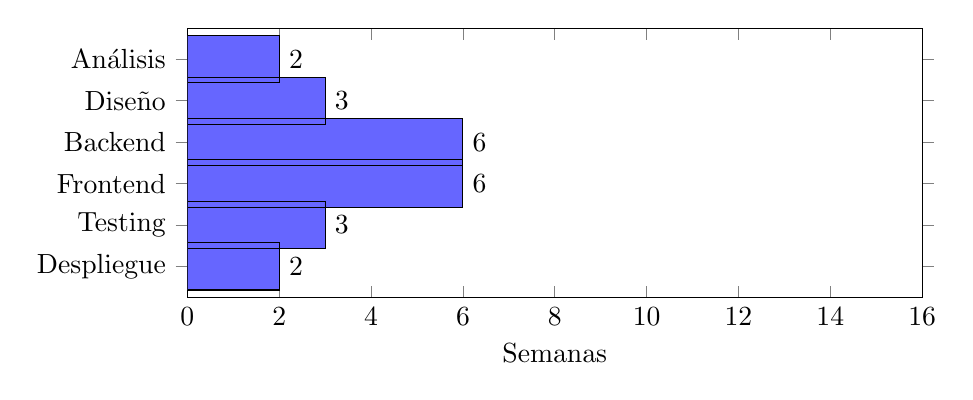
\begin{tikzpicture}
    \begin{axis}[
      width=0.9\textwidth,
      height=5cm,
      xbar,
      xlabel={Semanas},
      ytick={1,2,3,4,5,6},
      yticklabels={Despliegue,Testing,Frontend,Backend,Diseño,Análisis},
      xmin=0, xmax=16,
      bar width=0.6cm,
      nodes near coords,
      nodes near coords align={horizontal},
      enlarge y limits=0.15,
    ]
    % Duración de cada tarea (inicio implícito desde 0 para simplificar)
    \addplot[fill=blue!60] coordinates {(2,6) (3,5) (6,4) (6,3) (3,2) (2,1)};
    \end{axis}
  \end{tikzpicture}
  \caption{Diagrama de Gantt simplificado del proyecto}
  \label{fig:gantt-simple}
\end{figure}

\section{Tabla de resumen de resultados}
\label{sec:tabla-resumen}

Para finalizar, es común presentar un resumen numérico de los resultados:

\begin{table}[H]
  \centering
  \caption{Resumen de métricas de evaluación}
  \label{tab:resumen-metricas}
  \begin{tabular}{@{}lccccc@{}}
    \toprule
    \textbf{Métrica} & \textbf{Baseline} & \textbf{Propuesta} & \textbf{Mejora} & \textbf{p-valor} & \textbf{Sig.} \\
    \midrule
    Precisión & 78.5\% & 89.2\% & +10.7\% & 0.001 & *** \\
    Recall & 72.3\% & 86.8\% & +14.5\% & 0.003 & ** \\
    F1-Score & 75.2\% & 87.9\% & +12.7\% & 0.002 & ** \\
    Tiempo (ms) & 145 & 98 & -32.4\% & 0.015 & * \\
    Memoria (MB) & 512 & 384 & -25.0\% & 0.042 & * \\
    \bottomrule
  \end{tabular}

  \medskip
  \footnotesize
  Significancia: *** p < 0.001, ** p < 0.01, * p < 0.05
\end{table}

%% =============================================================================
\section{Anotaciones TikZ sobre imágenes}
\label{sec:anotaciones-tikz}

TikZ permite superponer elementos gráficos (flechas, círculos, etiquetas) sobre imágenes importadas. Esta técnica es muy útil para señalar partes específicas de fotografías, capturas de pantalla o diagramas.

\subsection{Técnica básica de superposición}
\label{subsec:superposicion-basica}

El método consiste en colocar la imagen dentro de un nodo TikZ y luego usar las coordenadas relativas para posicionar las anotaciones:

\begin{verbatim}
\begin{tikzpicture}
  % Imagen como nodo base
  \node[inner sep=0] (img)
    {\includegraphics[width=8cm]{imagen}};

  % Anotaciones usando coordenadas relativas
  \draw[red, thick, ->] (img.center) -- ++(1,1)
    node[above] {Etiqueta};
\end{tikzpicture}
\end{verbatim}

\subsection{Ejemplo de imagen con anotaciones}
\label{subsec:ejemplo-anotaciones}

El siguiente ejemplo muestra cómo señalar diferentes regiones de una imagen:

\begin{figure}[H]
  \centering
  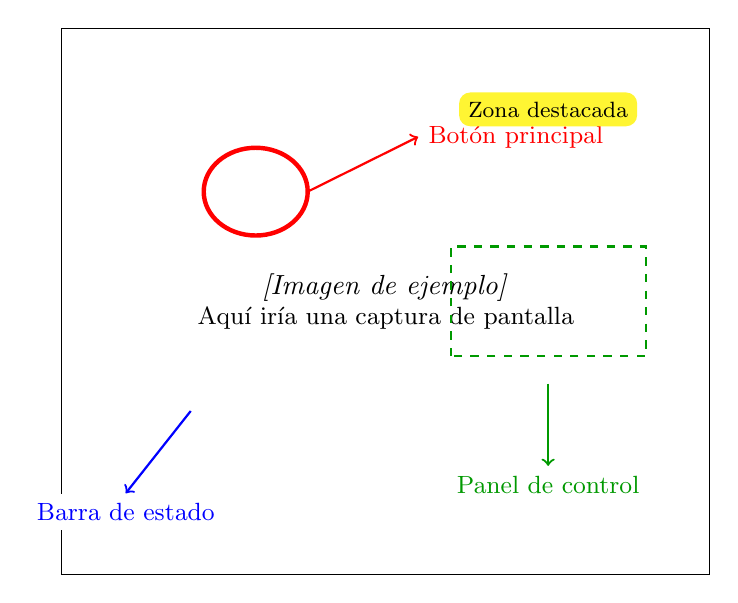
\begin{tikzpicture}
    % Imagen base (usando example-image como placeholder)
    \node[inner sep=0, anchor=south west] (img) at (0,0) {%
      \fbox{\parbox{8cm}{\centering\vspace{3cm}\textit{[Imagen de ejemplo]}\\\small Aquí iría una captura de pantalla\vspace{3cm}}}%
    };

    % Obtener dimensiones de la imagen
    \begin{scope}[x={(img.south east)}, y={(img.north west)}]
      % Círculo rojo señalando una zona
      \draw[red, ultra thick] (0.3, 0.7) circle (0.08);
      \draw[red, thick, ->] (0.38, 0.7) -- (0.55, 0.8)
        node[right, fill=white, font=\small] {Botón principal};

      % Flecha azul señalando otra zona
      \draw[blue, thick, ->] (0.2, 0.3) -- (0.1, 0.15)
        node[below, fill=white, font=\small] {Barra de estado};

      % Rectángulo verde destacando un área
      \draw[green!60!black, thick, dashed]
        (0.6, 0.4) rectangle (0.9, 0.6);
      \draw[green!60!black, thick, ->] (0.75, 0.35) -- (0.75, 0.2)
        node[below, fill=white, font=\small] {Panel de control};

      % Etiqueta con fondo
      \node[fill=yellow!80, rounded corners, font=\footnotesize]
        at (0.75, 0.85) {Zona destacada};
    \end{scope}
  \end{tikzpicture}
  \caption{Ejemplo de anotaciones sobre una imagen}
  \label{fig:imagen-anotada}
\end{figure}

\subsection{Anotaciones con numeración}
\label{subsec:anotaciones-numeradas}

Para documentación técnica, es común usar marcadores numerados:

\begin{figure}[H]
  \centering
  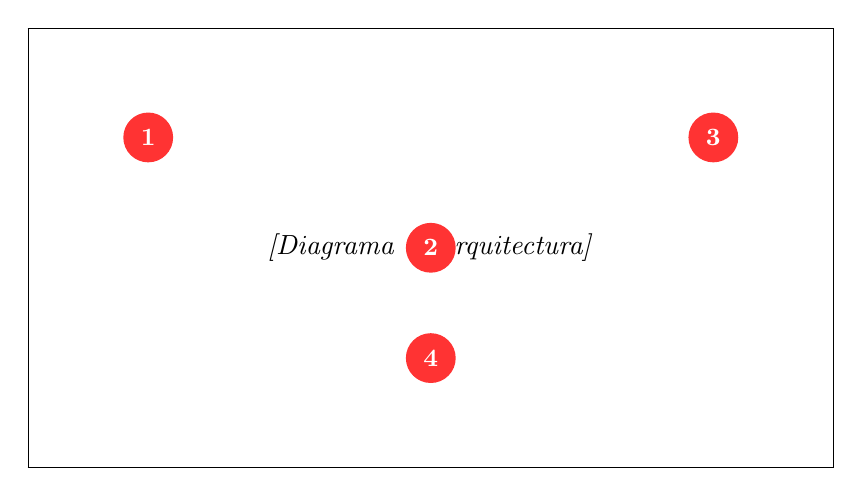
\begin{tikzpicture}
    % Imagen base simulada
    \node[inner sep=0, anchor=south west] (img) at (0,0) {%
      \fbox{\parbox{10cm}{\centering\vspace{2.5cm}\textit{[Diagrama de arquitectura]}\vspace{2.5cm}}}%
    };

    % Definir estilo para los marcadores
    \tikzset{
      marker/.style={
        circle, fill=red!80, text=white,
        font=\bfseries\small, inner sep=2pt, minimum size=18pt
      }
    }

    \begin{scope}[x={(img.south east)}, y={(img.north west)}]
      % Marcadores numerados
      \node[marker] at (0.15, 0.75) {1};
      \node[marker] at (0.5, 0.5) {2};
      \node[marker] at (0.85, 0.75) {3};
      \node[marker] at (0.5, 0.25) {4};
    \end{scope}
  \end{tikzpicture}

  \vspace{0.5em}
  \begin{enumerate}[leftmargin=2cm]
    \item \textbf{Frontend:} Interfaz de usuario React/Vue
    \item \textbf{API Gateway:} Punto de entrada de peticiones
    \item \textbf{Backend:} Servicios de lógica de negocio
    \item \textbf{Base de datos:} Almacenamiento persistente
  \end{enumerate}
  \caption{Arquitectura del sistema con marcadores explicativos}
  \label{fig:arquitectura-numerada}
\end{figure}

%% =============================================================================
\section{Diseños gráficos con TikZ}
\label{sec:disenos-tikz}

TikZ permite crear ilustraciones vectoriales de alta calidad directamente en el documento. A continuación se muestran ejemplos de diseños comunes.

\subsection{Formas geométricas básicas}
\label{subsec:formas-basicas}

\begin{figure}[H]
  \centering
  \begin{tikzpicture}
    % Rectángulo con esquinas redondeadas
    \draw[fill=blue!30, rounded corners=5pt] (0,0) rectangle (2,1.5);
    \node at (1, 0.75) {Caja};

    % Círculo con gradiente
    \shade[ball color=red!60] (4,0.75) circle (0.7);
    \node[white] at (4, 0.75) {Esfera};

    % Elipse
    \draw[fill=green!40, thick] (7,0.75) ellipse (1 and 0.6);
    \node at (7, 0.75) {Elipse};

    % Polígono regular (hexágono)
    \node[regular polygon, regular polygon sides=6,
          fill=orange!50, minimum size=1.5cm] at (10, 0.75) {Hex};
  \end{tikzpicture}
  \caption{Formas geométricas básicas en TikZ}
  \label{fig:formas-basicas}
\end{figure}

\subsection{Diagrama de flujo}
\label{subsec:diagrama-flujo}

Los diagramas de flujo son fundamentales para documentar procesos y algoritmos:

\begin{figure}[H]
  \centering
  \begin{tikzpicture}[
    node distance=1.2cm,
    startstop/.style={rectangle, rounded corners, fill=red!30,
                      draw, minimum width=2.5cm, minimum height=0.8cm},
    process/.style={rectangle, fill=blue!20, draw,
                    minimum width=2.5cm, minimum height=0.8cm},
    decision/.style={diamond, fill=green!20, draw,
                     aspect=2, minimum width=2cm},
    arrow/.style={thick, ->, >=stealth}
  ]
    % Nodos
    \node[startstop] (start) {Inicio};
    \node[process, below of=start] (input) {Leer datos};
    \node[decision, below of=input, yshift=-0.5cm] (decide) {¿Válido?};
    \node[process, below of=decide, yshift=-0.5cm] (process) {Procesar};
    \node[process, right of=decide, xshift=2.5cm] (error) {Mostrar error};
    \node[startstop, below of=process] (stop) {Fin};

    % Flechas
    \draw[arrow] (start) -- (input);
    \draw[arrow] (input) -- (decide);
    \draw[arrow] (decide) -- node[left] {Sí} (process);
    \draw[arrow] (decide) -- node[above] {No} (error);
    \draw[arrow] (error) |- (input);
    \draw[arrow] (process) -- (stop);
  \end{tikzpicture}
  \caption{Diagrama de flujo de validación de datos}
  \label{fig:diagrama-flujo}
\end{figure}

\subsection{Diagrama de bloques}
\label{subsec:diagrama-bloques}

Útil para representar sistemas y sus componentes:

\begin{figure}[H]
  \centering
  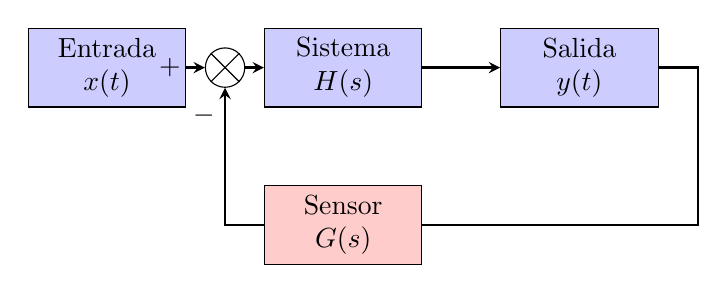
\begin{tikzpicture}[
    block/.style={rectangle, draw, fill=blue!20,
                  minimum width=2cm, minimum height=1cm, align=center},
    arrow/.style={thick, ->, >=stealth},
    line/.style={thick}
  ]
    % Bloques
    \node[block] (input) {Entrada\\$x(t)$};
    \node[block, right of=input, xshift=2cm] (system) {Sistema\\$H(s)$};
    \node[block, right of=system, xshift=2cm] (output) {Salida\\$y(t)$};

    % Bloque de realimentación
    \node[block, below of=system, yshift=-1cm, fill=red!20] (feedback) {Sensor\\$G(s)$};

    % Suma
    \node[circle, draw, left of=system, xshift=-0.5cm, minimum size=0.5cm] (sum) {};
    \draw (sum.north east) -- (sum.south west);
    \draw (sum.north west) -- (sum.south east);

    % Conexiones
    \draw[arrow] (input) -- (sum);
    \draw[arrow] (sum) -- (system);
    \draw[arrow] (system) -- (output);
    \draw[line] (output.east) -- ++(0.5,0) |- (feedback.east);
    \draw[arrow] (feedback.west) -| (sum.south) node[pos=0.9, left] {$-$};
    \node[left of=sum, xshift=0.3cm] {$+$};
  \end{tikzpicture}
  \caption{Diagrama de bloques de un sistema de control}
  \label{fig:diagrama-bloques}
\end{figure}

\subsection{Línea de tiempo}
\label{subsec:linea-tiempo}

Para representar cronologías o secuencias de eventos:

\begin{figure}[H]
  \centering
  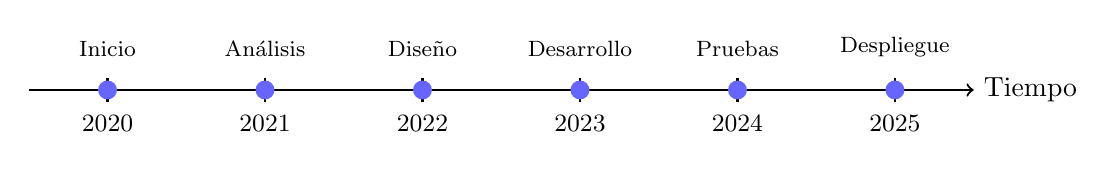
\begin{tikzpicture}
    % Línea principal
    \draw[thick, ->] (0,0) -- (12,0) node[right] {Tiempo};

    % Marcas y etiquetas
    \foreach \x/\year/\event in {
      1/2020/Inicio,
      3/2021/Análisis,
      5/2022/Diseño,
      7/2023/Desarrollo,
      9/2024/Pruebas,
      11/2025/Despliegue
    } {
      \draw[thick] (\x, 0.15) -- (\x, -0.15);
      \node[below, font=\small] at (\x, -0.2) {\year};
      \node[above, font=\footnotesize, text width=1.5cm, align=center]
        at (\x, 0.3) {\event};
      \fill[blue!60] (\x, 0) circle (0.12);
    }
  \end{tikzpicture}
  \caption{Línea de tiempo del proyecto}
  \label{fig:linea-tiempo}
\end{figure}

\subsection{Iconos y símbolos personalizados}
\label{subsec:iconos-simbolos}

TikZ permite crear iconos y símbolos vectoriales reutilizables:

\begin{figure}[H]
  \centering
  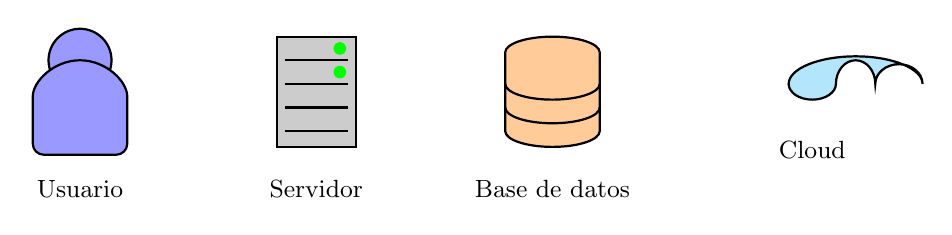
\begin{tikzpicture}
    % Icono de usuario
    \begin{scope}[shift={(0,0)}]
      \draw[fill=blue!40, thick] (0,0.3) circle (0.4);
      \draw[fill=blue!40, thick, rounded corners]
        (-0.6,-0.9) -- (-0.6,-0.3) arc (180:0:0.6) -- (0.6,-0.9) -- cycle;
      \node[below] at (0, -1.1) {\small Usuario};
    \end{scope}

    % Icono de servidor
    \begin{scope}[shift={(3,0)}]
      \draw[fill=gray!40, thick] (-0.5,-0.8) rectangle (0.5,0.6);
      \foreach \y in {0.3, 0, -0.3, -0.6} {
        \draw[thick] (-0.4, \y) -- (0.4, \y);
      }
      \fill[green] (0.3, 0.45) circle (0.08);
      \fill[green] (0.3, 0.15) circle (0.08);
      \node[below] at (0, -1.1) {\small Servidor};
    \end{scope}

    % Icono de base de datos
    \begin{scope}[shift={(6,0)}]
      \draw[fill=orange!40, thick] (0,0.4) ellipse (0.6 and 0.2);
      \draw[fill=orange!40, thick] (-0.6,0.4) -- (-0.6,-0.6)
        arc (180:360:0.6 and 0.2) -- (0.6,0.4);
      \draw[thick] (-0.6, 0) arc (180:360:0.6 and 0.2);
      \draw[thick] (-0.6, -0.3) arc (180:360:0.6 and 0.2);
      \node[below] at (0, -1.1) {\small Base de datos};
    \end{scope}

    % Icono de nube
    \begin{scope}[shift={(9,0)}]
      \draw[fill=cyan!30, thick]
        (0,0) arc (180:360:0.3 and 0.2)
        arc (180:0:0.25 and 0.3)
        arc (180:0:0.3 and 0.25)
        arc (0:180:0.85 and 0.35)
        -- cycle;
      \node[below] at (0.3, -0.6) {\small Cloud};
    \end{scope}
  \end{tikzpicture}
  \caption{Iconos vectoriales creados con TikZ}
  \label{fig:iconos-tikz}
\end{figure}

%% =============================================================================
\section{Diagramas de arquitectura}
\label{sec:diagramas-arquitectura}

\subsection{Arquitectura de microservicios}
\label{subsec:arquitectura-microservicios}

\begin{figure}[H]
  \centering
  \begin{tikzpicture}[
    service/.style={rectangle, draw, fill=blue!20, rounded corners,
                    minimum width=2cm, minimum height=0.8cm, font=\small},
    gateway/.style={rectangle, draw, fill=green!30, rounded corners,
                    minimum width=2.5cm, minimum height=0.8cm, font=\small},
    database/.style={cylinder, draw, fill=orange!30, shape aspect=0.3,
                     minimum width=1cm, minimum height=0.8cm, font=\footnotesize},
    client/.style={rectangle, draw, fill=gray!30, rounded corners,
                   minimum width=1.5cm, minimum height=0.6cm, font=\small},
    arrow/.style={->, thick, >=stealth}
  ]
    % Clientes
    \node[client] (web) at (0, 3) {Web};
    \node[client] (mobile) at (2, 3) {Móvil};
    \node[client] (api) at (4, 3) {API};

    % API Gateway
    \node[gateway] (gw) at (2, 1.5) {API Gateway};

    % Microservicios
    \node[service] (auth) at (-1, 0) {Auth};
    \node[service] (users) at (2, 0) {Users};
    \node[service] (orders) at (5, 0) {Orders};

    % Bases de datos
    \node[database] (db1) at (-1, -1.5) {DB};
    \node[database] (db2) at (2, -1.5) {DB};
    \node[database] (db3) at (5, -1.5) {DB};

    % Message Queue
    \node[rectangle, draw, fill=purple!20, minimum width=4cm] (mq)
      at (2, -3) {Message Queue};

    % Conexiones
    \draw[arrow] (web) -- (gw);
    \draw[arrow] (mobile) -- (gw);
    \draw[arrow] (api) -- (gw);
    \draw[arrow] (gw) -- (auth);
    \draw[arrow] (gw) -- (users);
    \draw[arrow] (gw) -- (orders);
    \draw[arrow] (auth) -- (db1);
    \draw[arrow] (users) -- (db2);
    \draw[arrow] (orders) -- (db3);
    \draw[arrow, dashed] (auth) |- (mq);
    \draw[arrow, dashed] (users) -- (mq);
    \draw[arrow, dashed] (orders) |- (mq);
  \end{tikzpicture}
  \caption{Arquitectura de microservicios}
  \label{fig:microservicios}
\end{figure}

\subsection{Diagrama de capas}
\label{subsec:diagrama-capas}

\begin{figure}[H]
  \centering
  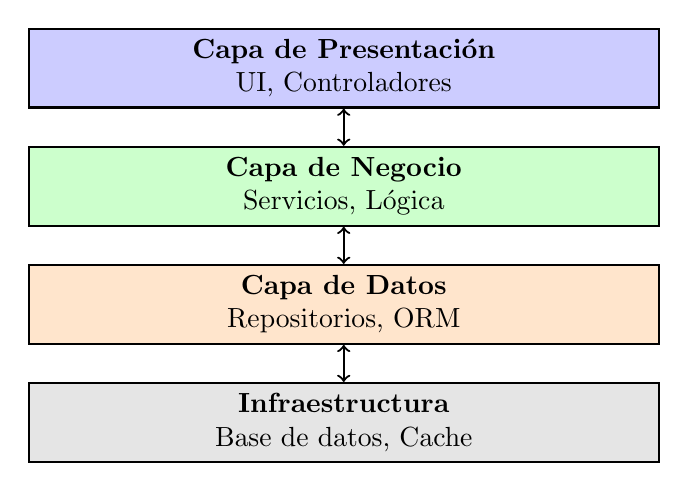
\begin{tikzpicture}
    \tikzset{
      layer/.style={rectangle, draw, thick, minimum width=8cm,
                    minimum height=1cm, align=center}
    }

    \node[layer, fill=blue!20] (pres) at (0, 3)
      {\textbf{Capa de Presentación}\\UI, Controladores};
    \node[layer, fill=green!20] (bus) at (0, 1.5)
      {\textbf{Capa de Negocio}\\Servicios, Lógica};
    \node[layer, fill=orange!20] (data) at (0, 0)
      {\textbf{Capa de Datos}\\Repositorios, ORM};
    \node[layer, fill=gray!20] (infra) at (0, -1.5)
      {\textbf{Infraestructura}\\Base de datos, Cache};

    % Flechas bidireccionales
    \draw[<->, thick] (pres.south) -- (bus.north);
    \draw[<->, thick] (bus.south) -- (data.north);
    \draw[<->, thick] (data.south) -- (infra.north);
  \end{tikzpicture}
  \caption{Arquitectura en capas}
  \label{fig:capas}
\end{figure}
